Plastic scintillators are organic scintillators that has been disolved in a solven and polimerized. They are easy to machine and can take any desired shape during construction. Among the forms most used today we can find blocks, thin sheets, cylinders, etc.

In our experiment we have been working with an plastic scintillator in the form of fiber, specifically, commercial fibers BCF-12 from Saint-Gobain Crystals Inc \cite{DataSheetBCF12Fiber}. This type of fiber was chosen as the result of a comparative study among some of the best-known commercial manufacturers, such as Kuraray \cite{DataSheetKuraray}. 

The BCF-12 fibers consist of a scintillated core, whose material is polystyrene, one of the most used solvents for plastic scintillators \cite{Knoll}, with the posibility of surounding it of a cladding of polymethylmethacrylate (PMMA) (smaller refractive index than core in order to archieve a critical angle) or a multicladding (second cladding) with even smaller refractive index.

When a particle deposits all or part of its kinetic energy, some photons are produced in the fiber core as a result of the scintillating process. The quantity of photons which are produced depend on the scintillation yield, whose value is around $8000$ photons per $\MeV$ for a mip in our case (BCF-12 fibers) . It means that, for instance, for tritium electron, this fibers will release a maximum of around 148 photons (when tritium electron has the maximum energy, $18.6~\keV$), probably less because electrons with these energies are not mips.

These photons will shape the useful part of the response of the scintillator (fluorescence) for us. The energy (or wavelength) of these scintillated photons follows the distribution of their emission spectrum which, for the used fibers, is shown in the figure \ref{fig:EmissionSpectrumFibers}.

\begin{figure}[htbp]
\centering
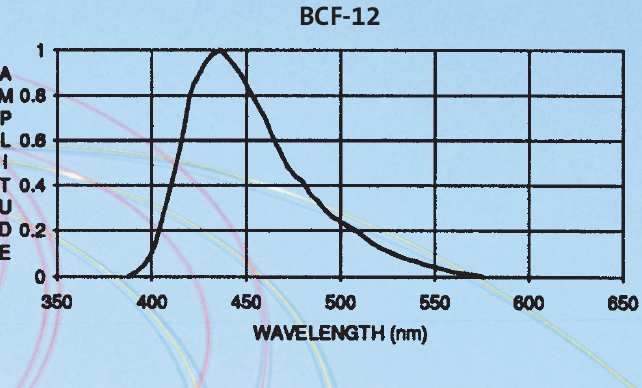
\includegraphics[scale=0.5]{3DesignPrinciples/32Tritium_detector/EmisionBCF12.png}
\caption{Emission spectrum of BCF-12 fibers of Saint-Gobain.\label{fig:EmissionSpectrumFibers}~\cite{DataSheetBCF12Fiber}}
\end{figure}

After the production of scintillated photons, we need to guide these photons to the sensitive part of the photosensor where we will detect them with some probability. Fibers (and scintillators in general) use the optical property of Snell's law \cite{Snell} to guide their photons to the desired part (the ends of the fibers). It is based on the interface created between the core and the surrounding material. When a photon hits this interface, it is refracted (and therefore lost) following the Snell equation, \ref{eq:Snell}. If the surrounding material has a lower index of refraction than the core of the fiber, there exist a critical angle, $\theta_c$, at which, for angles equal or larger than this one, the photons will be totally refracted (and therefore conserved in the fiber for being guided). This effect is showed in the figure \ref{fig:Fiber_physic}.

\begin{equation}
n_0~sen(\theta_0) = n_1~sen(\theta_1) \longrightarrow \theta_c = asen\left(\frac{n_1}{n_0} \right)
\label{eq:Snell}
\end{equation}

There exist a parameter which define the efficiency of the scintillator in order to guide photons, the trapping efficiency. For BCF-12 fibers is between $3.44\%$ and $7\%$ (depending if the event was detected near the fiber axis (minimum) or near the core-clad interface(maximum)).

Therefore, from these $148$ photons initially created with the tritium electron with the maximum energy, only a maximum of around 10 photons (for maximum trapping efficiency) will arrive to our photosensor. As you can see, we work with very weak detector signals, where there is more electronic noise and, as you will see in future chapters, we have made a big effort to reduce this electronic noise as much as possible with several technics.

In the figure \ref{fig:Fiber_physic} we can see how a scintilalting fiber works.

\begin{figure}[htbp]
\centering
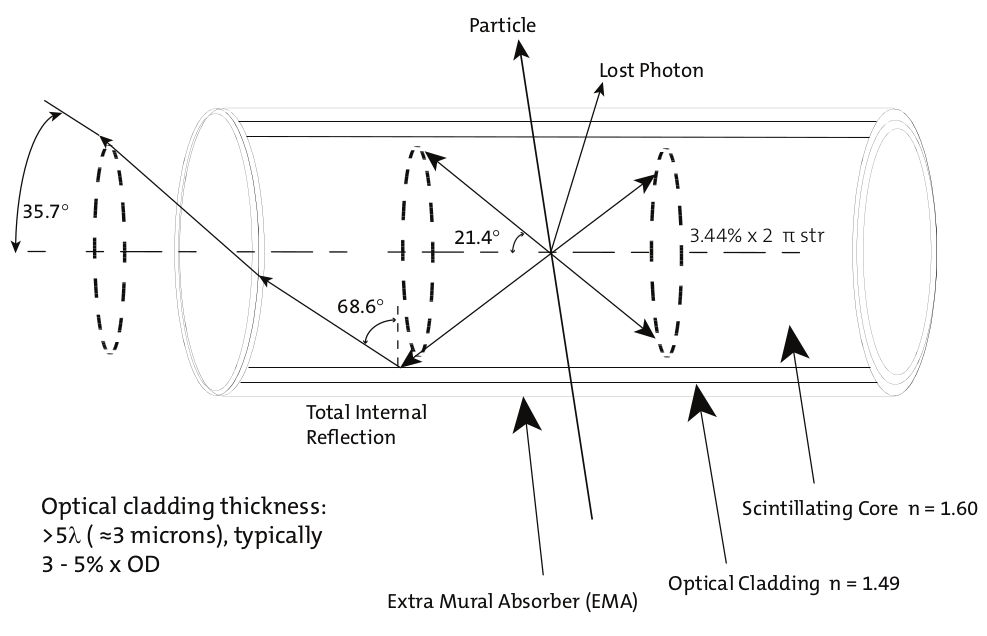
\includegraphics[scale=0.5]{3DesignPrinciples/32Tritium_detector/Fiber_data_sheet.png}
\caption{How photons are collected in a fiber with single clad.\label{fig:Fiber_physic}~\cite{DataSheetBCF12Fiber}}
\end{figure}

The cladding material is useful for protecting the core surface from dirt or aggressive external agents that can reduce the light collection but at the cost of losing some light because it increase the critical angle. In the table \ref{tab:CriticalAngles} we have three different examples where this effect is ilustrated.

\begin{table}[htbp]
%%\centering
\begin{center}
\begin{tabular}{|c|c|c|}
\hline
Material & Refractive index & critical angle ($\degree$) \\
\hline \hline \hline
Air & 1 & $42.98$ \\ \hline
Water & 1.33 & $62.47$ \\ \hline
Cladding of PMMA & 1.49 & $76.26$ \\ \hline
\end{tabular}
\caption{Critical angles asociated to different interfaces created with polystyrene, $n_0=1.6$, and other materials}
\label{tab:CriticalAngles}
\end{center}
\end{table}

This is what theoretically happens but, in the practice, it's difficult to archieve a perfect air-core or water-core interface and it will affect to the light collection. Due to the reason that the commercial claddings are thicker ($30~\micro \meter$) than the mean free path of tritium in water ( around $5~\micro\meter$) we cannot use commercial cladding in our detector hence we will need to take special attencion for archieving a water-core interface enough good. As we will see in the section \ref{}, we have used a special protocol developed in the ICMOL (pie de pagina explicando que es el ICMOL) for preparing fibers before we use them for tritium detection.

Some of the most important properties of the used fibers are summarized in the table \ref{tab:ParametersFibersBCF12}.

\begin{table}[htbp]
%%\centering
\begin{center}
\begin{tabular}{|c|c|c|}
%\hline
%Material & Refractive index \\
\hline \hline 
Core material & Polystyrene \\ \hline
Core refractive index & 1.60 \\ \hline
Density & 1.05 \\ \hline
Cladding material & Acrylic (PMMA) \\ \hline
Cladding refractive index & 1.49 \\ \hline
Cladding thickness ($\mu\meter$) & 30 \\ \hline
Numerical aperture & 0.58 \\ \hline
Trapping efficiency & 3.44\% minimum \\ \hline
%No. of H atoms per cc (core) & $4.82 \cdot{} 10^{22}$ \\ \hline
%No. of C atoms per cc (core) & $4.85 \cdot{} 10^{22}$ \\ \hline
%No. of electrons per cc (core) & $3.4 \cdot{} 10^{23}$ \\ \hline
Radiation lenght (cm) & 42 \\ \hline
Emission peak (nm) & 435 (Blue) \\ \hline
Decay Time, (ns) & 3.2 \\ \hline
1/e Length (m) & 2.7 \\ \hline
Scintillator yield (\#$\gamma$/MeV) & $\sim 8000$ \\ \hline
Operating Temperature & $-20\degree C$ to $50\degree C$ \\ \hline
\end{tabular}
\caption{Properties of BCF-12 fibers from Saint-Gobain Inc. \cite{DataSheetBCF12Fiber}}
\label{tab:ParametersFibersBCF12}
\end{center}
\end{table}

%Bunch -> manojo de fibras

%bundle -> haz de fibras